\subsection{Topologien}\label{ss:Topologien}

Bei einem Aufbau eines Sensornetzes stellt sich grundsätzlich die Frage, wie die einzelnen Sensoren miteinander Verbindungen aufbauen und kommunizieren sollen. Ein solche Verbindungsstruktur nennt sich in der Informatik 'Topologie'. Da das Sensornetz insgesamt zuverlässig arbeiten soll, Kosten und Komplexität jedoch gering gehalten werden sollen, wurden speziell für die drahtlosen Sensornetze neue Ansätze im Bereich der Topologie erforscht. Im folgenden sollen 4 Topologie-Alternativen näher erläutert werden. \\

Peer-to-Peer Netzwerke erlauben es, das jeder Knoten im Netz (in unserem Fall der Sensor) mit jedem anderen Knoten direkt Kontakt aufnehmen kann. Jedes 'Peer-Gerät' ist gleichzeitig Client und Server gegenüber anderen Knoten im Netzwerk.\\

\begin{figure}[H] 
	\centering
	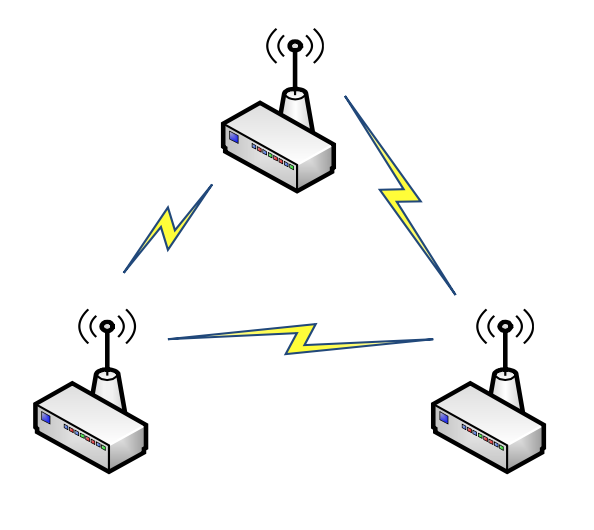
\includegraphics[scale=0.5]{Bilder/peertopeer}
	\caption{Peer-To-Peer Netzwerk\cite{d:kosmerchock}}
	\label{f:peertopeer}
\end{figure}

Bei der Stern-Topologie sind die Sensoren an ein zentrales Kommunikationsgerät angebunden. In diesem Fall kommunizieren die einzelnen Knoten nicht direkt miteinander. Jegliche Art von Kommunikation wird über das zentrale Gerät (auch Hub genannt) geroutet. Der Hub wird hier als Server betrachtet, wohingegen die Knoten (Sensoren) die Clients darstellen. \\

\begin{figure}[H] 
	\centering
	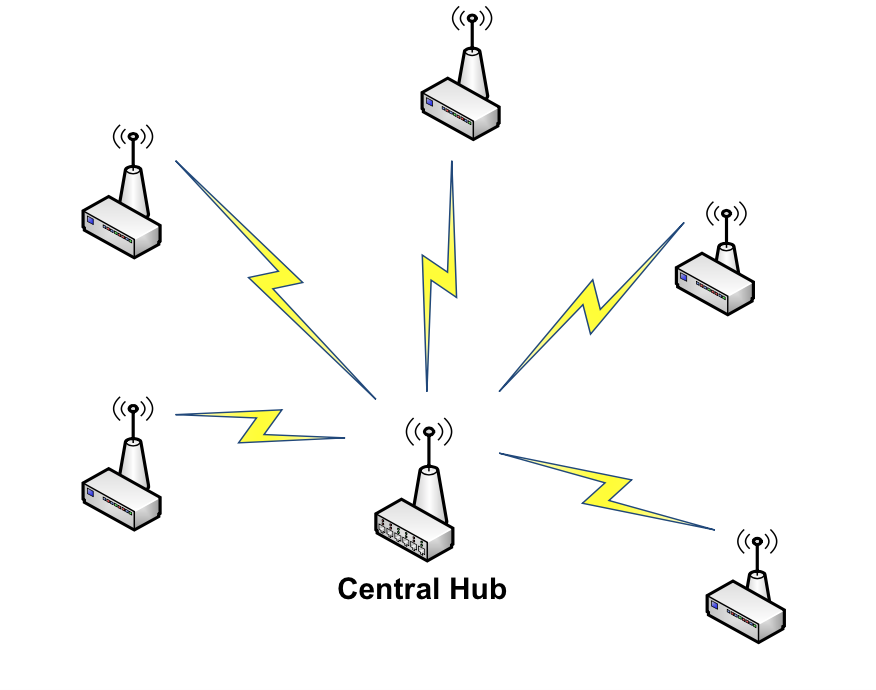
\includegraphics[scale=0.5]{Bilder/star}
	\caption{Stern Netzwerk\cite{d:kosmerchock}}
	\label{f:star}
\end{figure}

Die Baum-Topologie stellt eine Hybridvariante aus Peer-to-Peer und Stern-Topologie dar. Sie nutzt einen sogenannten 'Root-Knoten' als zentraler Router. Eine Ebene darunter liegen die Hubs, an denen wie in der Stern-Topologie die Sensoren angebunden sind. \\

\begin{figure}[H] 
	\centering
	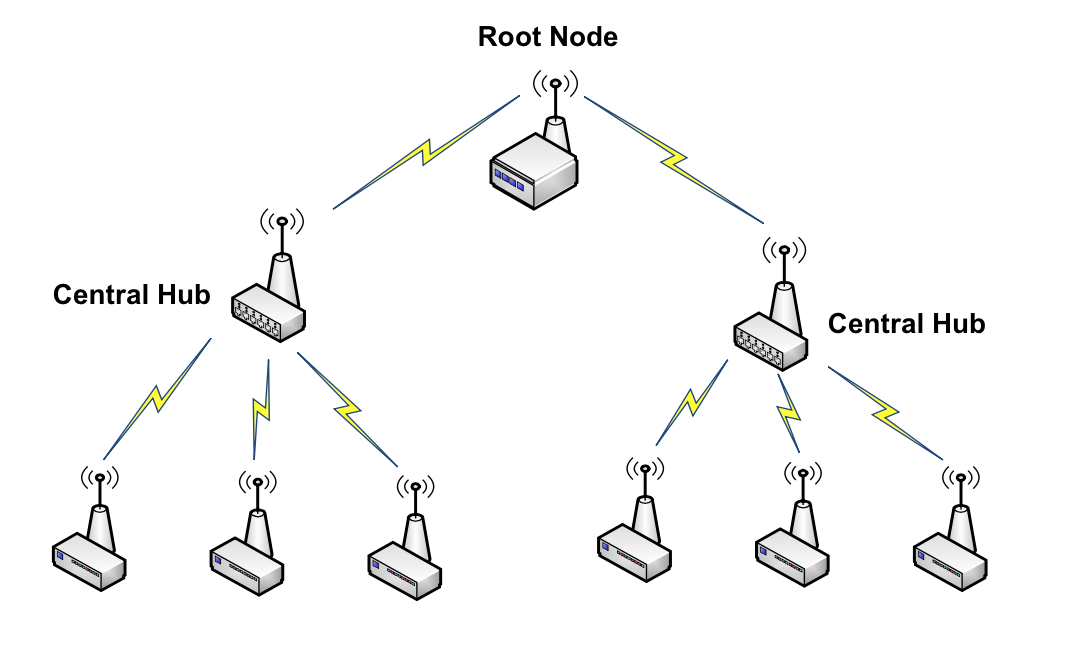
\includegraphics[scale=0.5]{Bilder/tree}
	\caption{Baum Netzwerk\cite{d:kosmerchock}}
	\label{f:tree}
\end{figure}

Eine weitere mögliche Variante ist ein vermaschtes Netz. Die Knoten sind untereinander ohne zentralen Hub verbunden und die Daten werden einfach von Knoten zu Knoten weitergesendet, bis sie ihr gewünschtes Ziel erreicht haben \cite{d:kosmerchock}. 

\begin{figure}[H] 
	\centering
	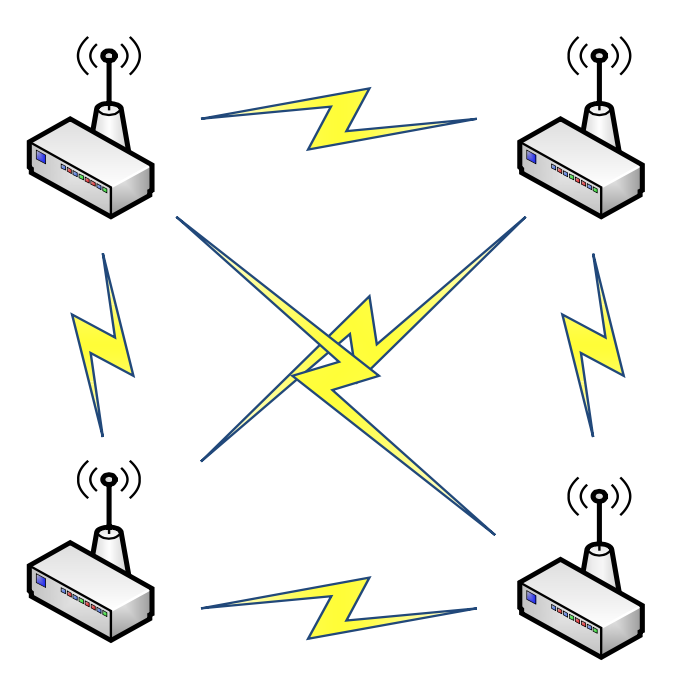
\includegraphics[scale=0.5]{Bilder/mesh}
	\caption{Vermaschtes Netzwerk\cite{d:kosmerchock}}
	\label{f:mesh}
\end{figure}